\chapter{Objetivos}
El objetivo de este proyecto será el de comprobar cómo la tecnología \textit{blockchain} puede servir para mitigar ataques a un esquema federado, concretamente a los ataques al modelo.

Para ello se analizará el estado actual de paradigma \textit{blockchain} aplicado al \ac{FL}, se estudiará la viabilidad de las distintas propuestas en el campo como mecanismo de defensa y se propondrá una nueva arquitectura que mejore de algún modo las soluciones ya existentes.

Los requerimientos del proyecto que desarrollemos se resumen en:
\begin{enumerate}
    \item Estudio y escritura sobre el estado actual de \ac{FL}.
    \item Estudio y escritura sobre la tecnología \textit{blockchain}.
    \item Estudio y escritura sobre la combinación y aplicabilidad de \ac{FL} y \textit{blockchain}.
    \item Implementar experimentos para comprobar la viabilidad de las propuestas.
    \item Estudio de una base matemática del trabajo.
    \item Escritura de la base matemática del trabajo.
    \item Estudio de los fundamentos de \textit{deep learning}.
    \item Redacción de los fundamentos de \textit{deep learning}.
    \item Análisis y escritura de los resultados y conclusiones del experimento.
\end{enumerate}

\chapter{Planificación y presupuesto}
Para mostrar como ha sido la planificación de tareas a lo largo del tiempo se ha hecho uso de un Diagrama de Gantt, una herramienta visual que permite ver la distribución de las tareas a lo largo de un periodo.

\begin{figure}[!h]
    \centering
    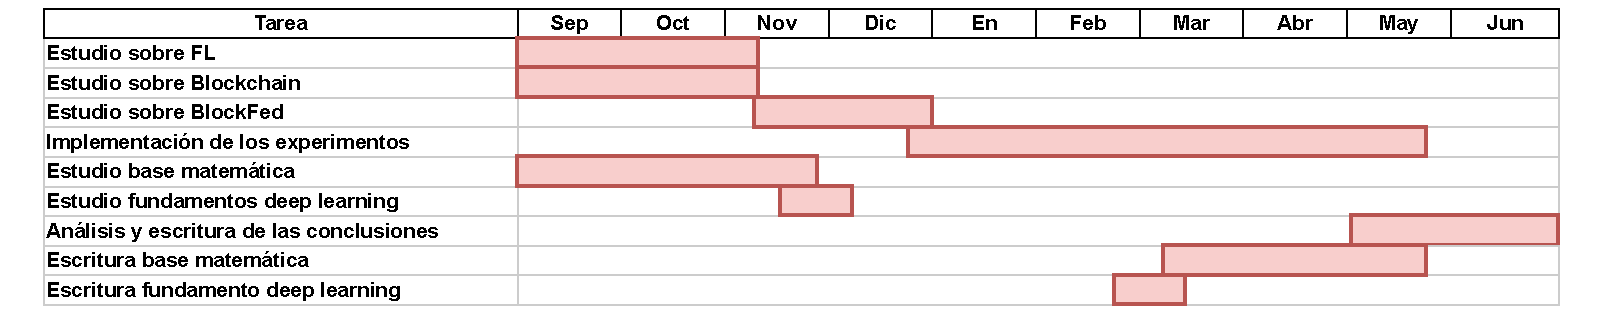
\includegraphics[width=\textwidth]{figuras/gantt.pdf}
    \caption{Diagrama de Gantt mostrando la planificación temporal.}
    \label{fig:gantt}
\end{figure}
Como podemos ver se ha trabajado de manera constante durante todo el curso en este trabajo. Las primeras tareas han sido la debida documentación sobre los fundamentos matemáticos, \ac{FL}, \textit{blockchain} y la aplicabilidad de estas dos tecnologías juntas. Durante el estudio de esta última, comenzó la implementación de los experimentos y su ejecución, la cuál ha ocupado gran parte en el tiempo debido a las múltiples iteraciones realizadas para verificar nuestras hipótesis. Una vez teniendo los experimentos encaminados, se ha dedicado el resto del tiempo a la escritura de la memoria y al análisis de estos.


En total se han empleado 10 meses para realizar el proyecto.


A la hora de calcular el presupuesto se tiene en cuenta los siguientes factores:
\begin{itemize}
    \item \textbf{Coste personal:} sabiendo que el sueldo medio de un Ingeniero Informático Jr. en España asciende a 1800 euros mensuales y su cotización social media es del 32,6\%, el gasto de personal de manera mensual sería de 2670,60 euros.

    Sabiendo la duración del proyecto y los datos anteriores deducimos que el gasto de personal para este proyecto es de $10 \times 2670,60=$ \textbf{26.706 euros}.

    \item \textbf{Coste del equipo:} para la realización de los experimentos se ha usado el clúster \textit{Talos} del Instituto Andaluz de Ciencia de Datos e Inteligencia Computacional (DaSCI) que destaca por contar con 8 tarjetas gráficas NVIDIA A100 40GB. Tras una aproximación del tiempo total de ejecución, el precio del uso de este clúster en un servicio como Google Cloud asciende a \textbf{4.601,35 euros}.
\end{itemize}

Por lo tanto, el presupuesto total de este trabajo sería de \textbf{31.307,35 euros}.